\section{Full EQ1 Derivation}
\label{app:eq1}

Let a single agent turn have:
\begin{itemize}
  \item $\Tdec$: main generation wall time (post-prefill, includes CoT and tool-call decode)
  \item $\Ttool$: tool execution wall time
  \item $\Tbase = \Tdec + \Ttool$: serial baseline cost
\end{itemize}
Under \spork{}, let $\alpha$ be the gate acceptance rate and $\toverlap$ be the mean realized overlap on accepted turns.

On \textbf{accepted turns} ($p = \alpha$), the speculative tool execution overlaps $\toverlap$ seconds of tool time with decode:
\[
  T_{\mathrm{hit}} = \Tbase - \toverlap
\]
On \textbf{rejected turns} ($p = 1 - \alpha$), the agent falls back to serial execution with overhead $\Toh$, but prefix recovery (D3) lets the main stream skip re-decoding the recovered tool-call tokens, replacing $\Tbase$ with the realized base cost $\Tbasestar = \Tbase - T_{\mathrm{D3}}$ ($\Tbasestar = \Tbase$ without D3):
\[
  T_{\mathrm{miss}} = \Tbasestar + \Toh
\]
Expected per-turn cost:
\[
  \begin{aligned}
  \mathbb{E}[T] &= \alpha \cdot T_{\mathrm{hit}} + (1-\alpha) \cdot T_{\mathrm{miss}} \\
                &= \Tbase - \alpha \cdot \toverlap + (1-\alpha)(\Tbasestar - \Tbase + \Toh)
  \end{aligned}
\]
Latency ratio:
\[
  S = \frac{\Tbase}{\Tbase - \alpha \cdot \toverlap + (1-\alpha) \cdot (\Tbasestar - \Tbase + \Toh)}
\]
For notational simplicity, the main text uses $\Tbasestar$ in place of $\Tbase$ on the speculative path and $\Toh$ as a uniform overhead (applied regardless of accept/reject), giving the formula $\Tbase / (\Tbasestar - \alpha \cdot \toverlap + \Toh)$.
The floor-2s validation in \S\ref{sec:envelope} uses this simplified form.

\paragraph{Break-even condition.}
$S \geq 1$ requires $\alpha \cdot \toverlap \geq (1-\alpha)(\Tbasestar - \Tbase + \Toh)$; without D3 ($\Tbasestar = \Tbase$) this reduces to $\alpha \cdot \toverlap \geq (1-\alpha) \cdot \Toh$, or approximately $\alpha \cdot \toverlap \geq \Toh$ when $\Toh$ is treated as a fixed overhead.

\paragraph{Tool-fraction ceiling.}
When $\alpha = 1$ and $\toverlap = \Ttool$ (perfect overlap of all tool time):
\[
  S_{\max} = \frac{\Tdec + \Ttool}{\Tdec} = \frac{1}{1 - \ftool}
\]
where $\ftool = \Ttool / \Tbase$ is the tool-time fraction.
On BrowseComp ($\ftool = 0.366$): $S_{\max} = 1.58\times$.
The gap between $S_{\max}$ and realized speedup is explained by (a) $\toverlap < \Ttool$ (probe dispatch lag + turns with $\Ttool < T_{\mathrm{probe}}$) and (b) $\Toh > 0$ on strict mode.

\section{D3 Partial-Token Accept: Phase 0 Data}
\label{app:d3}

Offline analysis of 1268 probe--baseline pairs from BrowseComp-120, a 120-question
probe-analysis run (distinct from the 240-question end-to-end evaluation run
described in Appendix~\ref{app:browsecomp}).
Both arms decode under identical observations, so the prefix statistics are
unbiased:

\begin{center}
\small
\begin{tabular}{lc}
\toprule
Statistic & Value \\
\midrule
Mean first-mismatch position $k$ & 29.5 tokens \\
Median $k$ & 27 tokens \\
$P_{25}$ / $P_{75}$ & 17 / 35 tokens \\
\% pairs with $k \geq 10$ & 82\% \\
\% pairs with $k \geq 20$ & 61\% \\
\bottomrule
\end{tabular}
\end{center}

Even rejected probes share a substantial token prefix with the baseline.
Accepting $k = 29.5$ tokens and autoregressively decoding the remaining $50 - 29.5 = 20.5$ tokens reduces the decode time of a full ${\sim}50$-token tool call from $\sim 1.5$\,s to $\sim 0.9$\,s (verify pass + 20.5 tokens), saving $\sim 0.6$\,s on such rejected turns.
In this 120-question run, 52\% of strict-gate turns were rejected, giving a mean per-turn D3 saving of $\approx 0.31$\,s.

\section{BrowseComp Experimental Details}
\label{app:browsecomp}

\paragraph{Setup.}
Qwen3-32B via vLLM 0.18.1, TP=4 on 4$\times$ NVIDIA H20-3e (143\,GiB each), bf16, max\_model\_len=40960.
BrowseComp first 240 questions (indices 0--239, fixed seed).
Temperature 0, seed 42 on all calls.
MAX\_TURNS = 15. Workers = 4 (4 questions in flight).
Tools: a production web-search API plus a web-page crawl/browse API.

\paragraph{First-token timeout.}
3.4\% of turns (50/1487) had probe dispatch timeout (first-token threshold = 3s).
These are treated as aborted probes; the turn falls back to serial execution.
Not catastrophic for overall results but indicates that under workers=4 concurrency, probe latency occasionally exceeds the 3s window on long real-content prompts.
D2 (confidence gating with earlier abort) would reduce this failure mode.

\paragraph{Fork statistics.}
\begin{center}
\small
\begin{tabular}{lc}
\toprule
Metric & Value \\
\midrule
Total tool turns & 1487 \\
Name hit rate & 83.7\% (1245/1487) \\
Args-exact rate & 38.8\% (577/1487) \\
Spec used (strict) & 577 (38.8\%) \\
Spec wasted (strict reject) & 687 (46.2\%) \\
First-token timeouts & 50 (3.4\%) \\
\bottomrule
\end{tabular}
\end{center}

\section{BrowseComp Timing Decomposition}
\label{app:timing}

Wall-time decomposition of the April HTTP-mode runs of Appendix~\ref{app:browsecomp};
the later engine-mode rerun shows the same tool share (37\%) but a larger prefill share
(it lacks the HTTP path's shared prefix cache).

\begin{center}
\resizebox{\columnwidth}{!}{%
\begin{tabular}{lcc}
\toprule
Component & Fraction of $\Tbase$ & Mean (s) \\
\midrule
$f_{\mathrm{tool}}$ (tool execution) & 36.6\% & 8.92 \\
$f_{\mathrm{dec}}$ (decode: CoT + tool\_call) & 57.2\% & -- \\
\quad CoT decode & 54.6\% & -- \\
\quad Tool-call decode & 2.6\% & -- \\
Other (prefill, overhead) & 6.2\% & -- \\
\midrule
Realized $\toverlap$ (spec\_used turns) & -- & 1.03 \\
Probe dispatch latency (mean probe\_wall) & -- & 0.72 \\
\bottomrule
\end{tabular}%
}
\end{center}

The 36\% turns with $\Ttool < 0.72$\,s (< probe\_wall) have zero realizable overlap: the tool completes before the probe can even dispatch speculative execution.
The 47\% turns with $\Ttool \in [0.72, 2]$\,s have limited overlap ($\leq 1.28$\,s).
Only the 17\% with $\Ttool \geq 2$\,s achieve substantial overlap.
Hence mean $\toverlap = 1.03$\,s despite mean $\Ttool = 8.92$\,s: 83\% of turns fall in the first two buckets.

\section{Per-Model Serving Configurations}
\label{app:configs}

Table~\ref{tab:benchmarks} profiles the three benchmarks of \S\ref{sec:setup};
Table~\ref{tab:configs} lists the serving mode, baseline, and \spork{} configuration
for every model in \S\ref{sec:experiments}.

\begin{table}[h]
\caption{\textbf{Benchmark and tool profile.} Tool vocabulary size, typical tool
latency, and turn depth per benchmark.}
\label{tab:benchmarks}
\centering
\footnotesize
\begin{tabular}{@{}lrrll@{}}
\toprule
Benchmark & N & \#Tools & Typical $\Ttool$ & Turns \\
\midrule
GAIA       & 165 & 2 & 4.8\,s mean (real)      & 1--8 \\
HotpotQA   & 200 & 1 & 0.9\,s mean (real)      & multi-hop \\
tau2-bench & 155 & 30 (2 dom.) & 0.5--5\,s floors (sim.) & multi-turn \\
\bottomrule
\end{tabular}
\end{table}
The HTTP configuration drives a stock vLLM server through its OpenAI-compatible API
and supports D1+D2 only; the engine configuration adds the D3 proposer integration
inside vLLM (\S\ref{sec:d3}).
Qwen3.5-35B-A3B uses JSON-format tool prompting throughout, as its native XML
tool-call format is a self-speculation boundary case (\S\ref{sec:envelope}).

\begin{table}[h]
\caption{\textbf{Per-model serving mode, baseline, and \spork{} configuration.}}
\label{tab:configs}
\centering
\footnotesize
\begin{tabular}{@{}llll@{}}
\toprule
Model & Serving mode & Baseline & \spork{} \\
\midrule
Qwen3-32B & engine & ngram spec.\ dec. & D1+D2+D3 \\
Qwen3-4B\textsuperscript{\dag} & engine & ngram spec.\ dec. & D1+D2+D3 \\
Qwen3.5-35B-A3B\textsuperscript{\ddag} & HTTP (JSON) & serial & D1+D2 \\
\bottomrule
\end{tabular}

\smallskip
{\footnotesize \textsuperscript{\dag}\,The tau2 run uses HTTP: serial baseline, D1+D2.
\textsuperscript{\ddag}\,The GAIA run uses D1 only.}
\end{table}

All end-to-end runs use greedy decoding with a fixed seed (42).

\section{Format-Divergence Boundary}
\label{app:format_divergence}

A model whose native tool-call format diverges from the forced probe defeats
self-speculation by collapsing the acceptance term ($\alpha \to 0$).
Qwen3.5-35B-A3B's native XML predicts the \emph{end-goal} tool rather than the next
intermediate one, collapsing fork-at-start name accuracy to
$\alpha_{\mathrm{name}}{=}4.5\%$ despite 97\% parse success; this is a semantic
next-step mismatch, not a parser failure, and it motivates the JSON-format prompting
of Table~\ref{tab:configs}.

\section{Qwen3-4B Full-Benchmark Coverage}
\label{app:qwen4b}

Figure~\ref{fig:qwen4b_coverage} and Table~\ref{tab:qwen4b_coverage} report the full
Qwen3-4B end-to-end coverage. These are
scaling-boundary diagnostics, not headline speedup claims: on the smaller model the
engine D1+D2+D3 protocol is near-neutral on HotpotQA and marginally positive on GAIA,
while the tau2 run (2\,s simulated tool-latency floor) shows a modest gain.
Even though Qwen3-4B in think mode produces long chains of thought (mean 3{,}323
CoT tokens on GAIA, 1{,}843 on HotpotQA), the smaller model decodes quickly, so the
overlap window and D3 recovery yield limited end-to-end benefit.

\begin{figure}[t]
  \centering
  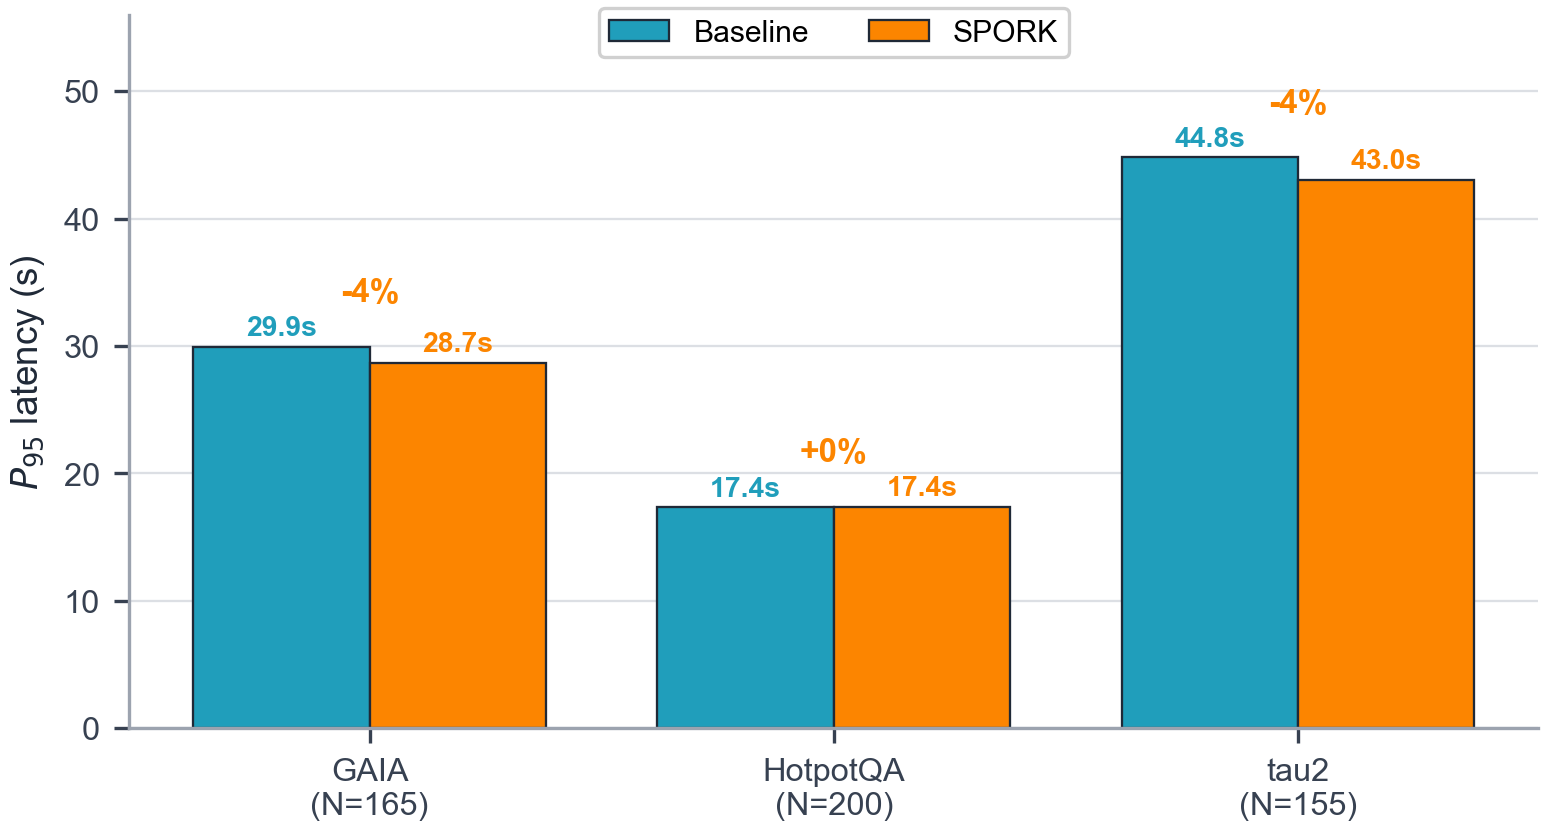
\includegraphics[width=\columnwidth]{figures/fig_qwen3_4b_coverage.png}
  \caption{\textbf{Qwen3-4B $P_{95}$ latency across benchmarks (scaling boundary).}
  \spork{} vs.\ baseline (GAIA/HotpotQA: engine D1+D2+D3 vs.\ ngram spec-dec; tau2:
  HTTP D1+D2 vs.\ serial). tau2 sees a modest gain, GAIA is marginally positive,
  and HotpotQA is neutral. Quality is preserved or improved (GAIA EM $29\to36/165$;
  HotpotQA EM $40\to39/200$, within $-$1\,pp).}
  \label{fig:qwen4b_coverage}
\end{figure}

\begin{table}[t]
  \centering
  \small
  \begin{tabular}{lrrrl}
    \toprule
    Benchmark & N & Baseline $P_{95}$ & \spork{} $P_{95}$ & Speedup \\
    \midrule
    GAIA      & 165 & 29.95\,s & 28.67\,s & 1.03$\times$ (agg) \\
    HotpotQA  & 200 & 17.36\,s & 17.39\,s & 1.00$\times$ (agg) \\
    tau2      & 155 & 44.81\,s & 43.04\,s & 1.15$\times$ (mean)$^{\dagger}$ \\
    \bottomrule
  \end{tabular}
  \caption{Qwen3-4B end-to-end results. Latency columns are $P_{95}$; the GAIA and
  HotpotQA speedups (agg) are aggregate wall-clock ratios on real tools.
  $^{\dagger}$tau2 reports the mean speedup at the 2\,s simulated tool-latency floor
  (21.2$\to$18.5\,s), not a $P_{95}$ ratio.}
  \label{tab:qwen4b_coverage}
\end{table}


\section{Late-Probe Supersession (\texttt{continue\allowbreak\_after\allowbreak\_dispatch})}
\label{app:supersede}

D2 issues a probe after each additional block of CoT, and Insight~2 shows that probe
accuracy rises as the chain-of-thought unfolds. This raises a design choice: should the
controller commit to the \emph{first} probe that clears the gate, or keep probing
and upgrade its speculation when a later, higher-confidence probe predicts a
different call? We expose this as a single switch, \texttt{continue\allowbreak\_after\allowbreak\_dispatch}:
\begin{itemize}
  \item \textbf{OFF (default):} the first probe that clears the confidence gate dispatches
        the speculative tool and the retry loop stops (first commit wins).
  \item \textbf{ON:} the controller keeps probing after dispatch; if a later probe predicts
        a different call, it cancels the in-flight speculative tool and re-dispatches the
        new candidate (a \emph{supersession}).
\end{itemize}

Table~\ref{tab:supersede} reports a controlled A/B on tau2 (Qwen3-32B, HTTP mode, 2\,s tool
floor, $N{=}30$, a subset of the 155-task suite, seed~42) using deterministic record$\to$replay tool execution so that tool
latency and output are identical across arms (zero cache-miss fallbacks). Supersession is
mildly beneficial: it raises the gate acceptance rate ($\alpha$ $0.714\to0.762$) and roughly
halves wasted speculative dispatches ($28\to15$) through 36 supersessions, with no latency
regression (mean wall $80.1\to77.5$\,s, within noise).

\begin{table}[t]
  \centering
  \small
  \begin{tabular}{lrrr}
    \toprule
    Config & $\alpha$ (used/disp.) & wasted disp. & superseded \\
    \midrule
    baseline      & --             & 0  & 0  \\
    OFF (first commit) & 0.714      & 28 & 0  \\
    ON (supersede)     & 0.762 & 15 & 36 \\
    \bottomrule
  \end{tabular}
  \caption{Effect of \texttt{continue\allowbreak\_after\allowbreak\_dispatch} on tau2 (Qwen3-32B, HTTP, 2\,s floor,
  $N{=}30$, deterministic replay).}
  \label{tab:supersede}
\end{table}

The effect is small enough that we leave \texttt{continue\allowbreak\_after\allowbreak\_dispatch} as an optional
knob rather than a headline mechanism, and the main-paper results use the default behavior.
We do not report a GAIA latency A/B for this switch: with real free-text search, the main
stream's queries diverge across arms (no API seed under concurrent main/probe decode), so a
clean replay is not possible in HTTP mode; an engine-mode deterministic harness would be
required.
